\chapter{Literature Review}

% TODO: consider which parts to move to chapter 3 ex. our calculations or conclusions

\section{CNN Model Design}

Different papers define and draw their CNN design differently,
this research analyses them then represent them into a unified table.

% TBD NOTE: in figures Convention input is put at the bottom and classes at the top or left to right.

\subsection{LeNet}

LeNet\autocite{lecun1998gradient} was one of the first successful ConvNets. 
It was used to recognize characters (thus domain specific),
the research was based on NIST Special Database 1 (SD-3)\autocite{wilson1990nist}
and NIST Special Database 3 (SD-3)\autocite{garris1992nist}
and their research resulted in one of the most infamous databases;
the Modified National Institute of Standards and Technology(MNIST) database\autocite{lecun2010mnist}.

Their CNN operates on a gray-scale input of 32×32 pixels (or 28×28 surrounded with 4 padding pixels),
input images were pre-processed to be centered, normalized, segmented ..etc.
First convolution is applied without padding, it has kernel size 5×5 (two pixels from each side around center)
which would output a volume of size 28×28. In the initial paper they used output
depth of 6 for the first convolution layer as shown in figure \ref{fig:lenet} from same paper.

In other words, first layer would train six kernels each of size 5×5 transforming
a volume of 32×32×1 input (depth is 1 not 3 because it's input is not colored)
into an output of 28×28×6.

LeNet-5 has seven layers as seen in figure \ref{fig:lenet},
five of them have trainable weights and two layers of them do not have weights.

Table \ref{table:lenet-cnn} demonstrates operations done on each layer and the corresponding number of parameters
to be trained (weight and bias values) and number of multiplications operations
(same number of addition operations) in each layer

\begin{figure}[!h]
\centering
\includegraphics[width=5in]{lenet}
\caption{LeNet-5 CNN desgin}\label{fig:lenet}
{Source: \autocite{lecun1998gradient}\hfill}
\end{figure}


\begin{table*}\caption{Details of LeNet layers, their input size, kernel size, output size and number of parameters (weights and bias).  W×H×D/S stands for width, height, depth and stride respectively}\label{table:lenet-cnn}
\centering
\begin{small}
\begin{tabularx}{\textwidth}{llllXX}
\toprule
Layer & Input & Kernel & Output & Params & Mults \\
Name & W×H×D & W×H×D/S & W×H×D & &  \\
\midrule
C1: conv2d & 32×32×1 & 5×5×6 &  28×28×6 & 1×5×5×6+6 =156 & 28×28×1×5×5×6 =117,600 \\
S2: pool/2 & 28×28×6 & 2×2/2 &  14×14×6 & 0 & 0 \\
C3: conv2d & 14×14×6 & 5×5×16 & 10×10×16 & 6×5×5×16+16 =2,416 & 10×10×6×5×5×16 =240,000 \\
S4: pool/2 & 10×10×16 & 2×2/2 &  5×5×16 & 0 & 0 \\
C5: conv2d & 5×5×16 & 5×5×120 &  1×1×120 & 16×5×5×120+120 =48,120 & 1×1×16×5×5×120 =48,000 \\
F6: conv2d & 1×1×120 & 1×1×84 &  1×1×84 & 120×1×1×84+84 =10,164 & 120×84 =10,080 \\
F7: conv2d & 1×1×84 & 1×1×10 &   1×1×10 & 84×1×1×10+10 =850 & 84×40 =840 \\
\cmidrule{4-6}
\multicolumn{4}{r}{Total} & 61,706 & 416,520 \\
\bottomrule
\end{tabularx}
\end{small}
\end{table*}

Despite having a simple design, shallow depth and specific simple task operating on a pre-processed normalized input,
it has more than 61k parameters and about half million multiplication operation and half million addition operations.
F6 is a fully connected hidden layer and F7 is the fully connected output layer,
the output depth of last layer is the number of classes in this example that is the ten digits from 0-9.
Another note that will be commonly seen in this research that most weights are in layer that flatten its input into 1×1 just before fully connected layers,
in LeNet it's C5 with 78\% of weights.

Note: Because bias values is very small compared to weights as we have seen above, we would only show weights. 

\subsection{AlexNet}

AlexNet\autocite{krizhevsky2012imagenet} was the winner of ILSVRC in 2012,
the design of this ConvNet is demonstrated in figure \ref{fig:alexnet} which shows half of it which is running
on one GPU having a similar copy runs on another GPU, for example, on the left it starts with an input image
and pass it through 11×11 kernel of depth 48 on one GPU and another same sized depth on the other GPU, 
resulting total of 96 filters to be learned. 

AlexNet main contribution is the use two GPUs in parallel with less communication between them
and the reduction of over-fitting with data augmentation and dropout.

\begin{figure}[!h]
\centering
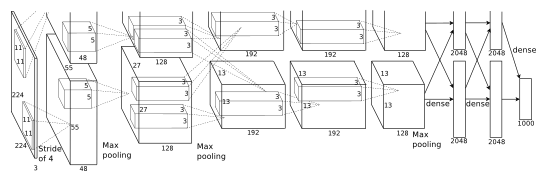
\includegraphics[width=5in]{alexnet}
\caption{AlexNet running on two GPU cores}\label{fig:alexnet}
{Source: \autocite{lecun1998gradient}\hfill}
\end{figure}

A slightly modified version of AlexNet (called AlexNet v2\autocite{krizhevsky2014one}) is shown
in the table \ref{table:alexnet-cnn}

\clearpage
\begin{landscape}
\clearpage
\centering

\begin{table*}\caption{Analysis of AlexNet v2 layers, showing input size, kernel size, output size and number of weights and multiplications and their percent. Kernel size is width, height, depth and stride in the form of WxHxD/S}\label{table:alexnet-cnn}
\centering
\begin{tabularx}{\hsize}{Xlllrrrr}
\toprule
Layer & Input & Kernel & Output & Weights & \% & Mults & \% \\
\midrule
c1: conv2d/4 & 224×224×3 & 11×11×64/4 & 54×54×64 & 3×11×11×64 & 0\% & 54×54×3×11×11×64 & 9.2\% \\
pool/2 & 54×54×64 & 3×3/2 & 26×26×64 & 0 & 0 & 0 & 0 \\
c2: conv2d & 26×26×64 & 5×5×192 & 26×26×192 & 64×5×5×192 & 0.6\% & 26×26×64×5×5×192 &  \textbf{28.2\%} \\
pool/2 & 26×26×192 & 3×3/2 & 12×12×192 & 0 & 0 & 0 & 0 \\
c3: conv2d & 12×22×192 & 3×3×384 & 12×12×384 & 192×3×3×384 & 1.3\% & 12×12×192×3×3×384 & 13.0\% \\
c4: conv2d & 12×12×384 & 3×3×384 & 12×12×384 & 384×3×3×384 & 2.6\% & 12×12×384×3×3×384 & 25.9\% \\
c5: conv2d & 12×12×384 & 3×3×256 & 12×12×256 & 384×3×3×384 & 1.8\% & 12×12×384×3×3×384 & 17.3\% \\
pool/2 & 12×12×256 & 3×3/2 & 5×5×256 & 0 & 0 & 0 & 0 \\
fc6 & 5×5×256  & 5×5×4096 & 1×1×4096 & 256×5×5×4096 &  \textbf{52.1\%} & 1×1×256×5×5×4096 & 3.6\% \\
fc7 & 1×1×4096 & 1×1×4096 & 1×1×4096 & 4096×1×1×4096 & 33.4\% & 4096×4096 & 2.3\% \\
fc8 & 1×1×4096 & 1×1×1000 & 1×1×1000 & 4096×1×1×1000 & 8.1\% & 4096×1000 & 0.6\% \\
\cmidrule{5-8}
\multicolumn{4}{r}{total} & 50M & 100\% & 737M & 100\% \\
\bottomrule
\end{tabularx}
\end{table*}

\end{landscape}
\clearpage

\subsection{ZFNet}

ZFNet\autocite{zeiler2014visualizing} (also known as Zeiler \& Fergus architecture)
was the winner of ILSVRC 2013. ZFNet's main contribution is the concept of ``DeConv'',
as they covered part of input image with a gray square to see which part of the image activates which part of the neural network.

This model is slightly modified Alexnet, same depth, same blocks with smaller stride of two at first convolution of four
and smaller filter size of 7 instead of 11, slightly more weights and operations,
for details refer to figure \ref{fig:zfnet} and table \ref{table:zfnet}.

\begin{figure}[!h]
\centering
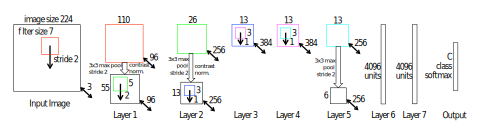
\includegraphics[width=5in]{zfnet}
\caption{ZFNet design}\label{fig:zfnet}
{Source: \autocite{zeiler2014visualizing}\hfill}
\end{figure}

\clearpage
\begin{landscape}
\clearpage
\centering

\begin{table*}\caption{Analysis of ZFNet layers}\label{table:zfnet}
\centering
\begin{tabularx}{\hsize}{Xlllrrrr}
\toprule
Layer & Input & Kernel & Output & Weights & \% & Mults & \% \\
\midrule
c1: conv2d/2 & 224×224×3 & 7×7×96/2 & 110×110×96 & 3×7×7×96 & 0.0\% & 110×110×3×7×7×96 & 14.6\% \\
pool/2 & 110×110×96 & 3×3/2 & 55×55×96 & 0 & 0.0\% & 0 & 0.0\% \\
c2: Conv2d/2 & 55×55×56 & 5×5×256 & 26×26×256 & 96×5×5×256 & 1.0\% & 26×26×96×5×5×256 & \textbf{35.6\%} \\
pool/2 & 26×26×256 & 3×3/2 & 13×13×256 & 0 & 0.0\% & 0 & 0.0\% \\
c3: conv2d & 13×13×256 & 3×3×384 & 13×13×384 & 256×3×3×384 & 1.4\% & 13×13×256×3×3×384 & 12.8\% \\
c4: conv2d & 13×13×384 & 3×3×384 & 13×13×384 & 384×3×3×384 & 2.1\% & 13×13×384×3×3×384 & 19.2\% \\
c5: conv2d & 13×13×384 & 3×3×256 & 13×13×256 & 384×3×3×256 & 1.4\% & 13×13×384×3×3×256 & 12.8\% \\
pool/2 & 13×13×256 & 3×3/2 & 6×6×256 & 0 & 0.0\% & 0 & 0.0\% \\
fc6 & 6×6×256 & 6×6×4096 & 1×1×4096 & 256×6×6×4096 & \textbf{60.5\%} & 256×6×6×4096 & 3.2\% \\
fc7 & 1×1×4096 & 1×1×4096 & 1×1×4096 & 4096×4096 & 26.9\% & 4096×4096 & 1.4\% \\
fc8 & 1×1×4096 & 1×1×1000 & 1×1×1000 & 4096×1000 & 6.6\% & 4096×1000 & 0.4\% \\
\cmidrule{4-8}
\multicolumn{4}{r}{Total} & 62M & 100\% & 1,168M & 100\% \\
\bottomrule
\end{tabularx}
\end{table*}

\end{landscape}
\clearpage

\subsection{VGG}
VGG\autocite{simonyan2014very} came second in ILSVRC 2014, 
The paper discussed many variations named after number of layers with trainable weights
for example VGG16 (variation D in the paper) have has 16 layers with trainable weights,
VGG-16 has 138M weights, 74\% of which are in ``fc6'' layer as seen in table \ref{table:vgg}.

VGG-16 was the best performing variation of VGG, It was better than shallower variations like VGG-11 (variation A)
and deeper variations like VGG-19 (variation E)

\clearpage
\begin{landscape}
\clearpage
\centering
\begin{table*}\caption{Analysis of VGG-16}\label{table:vgg}
\centering
\begin{tabularx}{\hsize}{Xlllrrrr}
\toprule
Layer & Input & Kernel/Stride & Output & Weights & \% & Mults & \% \\
\midrule
Name & Wi×Hi×Di & Wk×Hk×Do/S & Wo×Wo×Do & Wk×Hk×Do×Di & - & Wo×Ho×Wk×Hk×Do×Di & - \\
\midrule
conv1\_1 & 224×224×3 & 3×3×64 & 224×224×64 & 3×3×64×3 & 0.0\% &   224×224×3×3×64×3 & 0.6\% \\
conv1\_2 & 224×224×64 & 3×3×64 & 224×224×64 & 3×3×64×64 & 0.0\% & 224×224×3×3×64×64 & 12.0\% \\
pool/2 & 224×224×64 & 2×2/2 & 112×112×64 & 0 & 0 & 0 & 0 \\
conv2\_1 & 112×112×64  & 3×3×128 & 112×112×128 & 3×3×128×64 & 0.1\% & 112×112x3×3×128×64 & 6.0\% \\
conv2\_2 & 112×112×128 & 3×3×128 & 112×112×128 & 3×3×128×128 & 0.1\% & 112×112x3×3×128×128 & 12.0\% \\
pool/2 & 112×112×128 & 2×2/2 & 56×56×128 & 0 & 0 & 0 & 0 \\
conv3\_1 & 56×56×128 & 3×3×256 & 56×56×256 & 3×3×256×128 & 0.2\% & 56×56×3×3×256×128 & 6.0\% \\
conv3\_2 & 56×56×256 & 3×3×256 & 56×56×256 & 3×3×256×256 & 0.4\% & 56×56×3×3×256×128 & 12.0\% \\
conv3\_3 & 56×56×256 & 3×3×256 & 56×56×256 & 3×3×256×256 & 0.4\% & 56×56×3×3×256×128 & 12.0\% \\
pool/2 & 56×56×256 & 2×2/2 & 28×28×256 & 0 & 0 & 0 & 0 \\
conv4\_1 & 28×28×256 & 3×3×512 & 28×28×512 & 3×3×512×256 & 0.9\% & 28×28×3×3×512×256 & 6.0\% \\
conv4\_2 & 28×28×256 & 3×3×512 & 28×28×512 & 3×3×512×512 & 1.7\% & 28×28×3×3×512×512 & 12.0\% \\
conv4\_3 & 28×28×256 & 3×3×512 & 28×28×512 & 3×3×512×512 & 1.7\% & 28×28×3×3×512×512 & 12.0\% \\
pool/2 & 28×28×512 & 2×2/2 & 14×14×512 & 0 & 0 & 0 & 0\\
conv5\_1 & 14×14×512 & 3×3×512 & 14×14×412 & 3×3×512×512 & 1.7\% & 14×14×3×3×512×512 & 3.0\% \\
conv5\_2 & 14×14×512 & 3×3×512 & 14×14×412 & 3×3×512×512 & 1.7\% & 14×14×3×3×512×512 & 3.0\% \\
conv5\_3 & 14×14×512 & 3×3×512 & 14×14×412 & 3×3×512×512 & 1.7\% & 14×14×3×3×512×512 & 3.0\% \\
pool/2 & 14×14×512 & 2×2/2 & 7×7×512 & 0 &  0 & 0 & 0 \\
fc6: conv2d & 7×7×512 & 7×7×4096 & 1×1×4096 & 7×7×4096×512 & \textbf{74.3\%} & 7×7×4096×512 & 0.7\% \\
fc7: conv2d & 1×1×4096 & 1×1×4096 & 1×1×4096 & 4096×4096 & 12.1\% & 4096×4096 & 0.1\% \\
fc8: conv2d & 1×1×4096 & 1×1×1000 & 1×1×1000 & 4096×1000 & 3.0\% & 4096×1000 & 0.0\% \\
\cmidrule{4-8}
\multicolumn{4}{r}{Total:} & 138M & 100\% & 15,470M & 100\% \\
\bottomrule
\end{tabularx}
\end{table*}
\end{landscape}
\clearpage


\subsection{GoogLeNet or Inception v1}\label{sec_inception_v1}
GoogLeNet (aka \href{https://github.com/google/inception/blob/master/inception.ipynb}{Inception} v1)\autocite{szegedy2015going}, the winner of ILSVRC 2014,
has 22 layer having trainable weights (more than two times deeper than AlexNet v2\autocite{krizhevsky2014one}).
The design of this model is very different as input flows in branches that later get joined using ``DepthConcat''
which as its name suggests places collect the output of different branches along the depth of output volume.
That building block of this design is called ``inception module'' which is shown in figure \ref{fig:inception-block},
their CNN is composed of nine inception blocks
(not to be confused with layers).
Each block has four branches and it's two layers deep (except one branch, which has one layer)

\begin{itemize}
\item 1×1 followed by 3×3
\item 1×1 followed by 5×5
\item Max Pooling of size 3×3 (stride of 1) followed by 1×1
\item 1×1
\end{itemize}


\begin{figure}[!h]
\centering
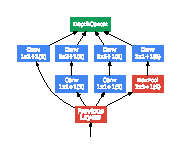
\includegraphics[width=5in]{inception-block}
\caption{An Inception module block}\label{fig:inception-block}
{Source: \autocite{szegedy2015going}\hfill}
\end{figure}


As mentioned before those branches are merged using ``depth concatenation'', for example first inception block takes
input of size 28×28×192 (coming from the output previous convolutions and pooling)
which flows to the four mentioned branches
the 1×1×64 branch outputs 28×28×64, the 3×3×128 branch outputs 28×28×128, the 5×5×32 branch outputs 28×28×32
and the max pool branch outputs 28×28×32 (because pooling stride is 1),
resulting matching output size of 28×28 and total number of depth to be \( 64+128+32+32 = 256 \) in depth.

Separable operators technique has been discussed previously and it's seen here,
instead of making a branch of 3×3×128,
they made it into 1×1×96 followed by 3×3×128 (here depth multiplier is 96).
The table \ref{table:inception-sep3} compares the 3×3 part of first inception block compared to its non-reduced equivalent,
using depth-multiplayer of 96 (reducing input depth from 192 to 96)
and as a result of this reduction number of weights were reduced by about 41.7\% and number of multiplications were reduced by about 41\%. 

Unlike separable operators we have seen before, the 1×1 point-wise stage is placed before the depth-wise stage in Inception.
Table \ref{table:inception-sep5} shows the 5×5 part of first inception block compared to its non-reduced equivalent,
using depth multiplier of 16 (reducing input depth from 192 to 16)
and as a result of this reduction number of weights were reduced by 90\%
and number of multiplications were reduced by 90\%. 


\begin{table*}\caption{Overhead of 3×3×128 convolution in Inception almost halved using separable operators}\label{table:inception-sep3}
\begin{small}
\begin{tabularx}{\textwidth}{ccccXX}
\toprule
\textbf{Name} & \textbf{Input} & \textbf{kernel} & \textbf{output} & \textbf{weights} & \textbf{mults} \\
\midrule
\multicolumn{6}{c}{Separable Version} \\
\midrule
point-wise & 28×28×192 & 1×1×96 & 28×28×96 & 1×1×96×192 & 28×28×96×192 \\
depth-wise & 28×28×96 & 3×3×128 & 28×28×128 & 3×3×128×96 & 28×28×3×3×128×96 \\
\cmidrule{4-6}
\multicolumn{3}{r}{} & \multicolumn{1}{l}{Total} & 129K & 101M \\
\midrule
\multicolumn{6}{c}{Non-separable Version} \\
\midrule
original & 28×28×192 & 3×3×128 & 28×28×128 & 3×3×128×192 =221K & 28×28×3×3×192×128 =173M \\
\bottomrule
\end{tabularx}
\end{small}
\end{table*}


\begin{table*}\caption{Overhead of 5×5×32 convolution in Inception reduce by 90\%}\label{table:inception-sep5}
\begin{small}
\begin{tabularx}{\textwidth}{ccccXX}
\toprule
Name & Input & kernel & output & weights & mults \\
\midrule
\multicolumn{6}{c}{Separable Version} \\
\midrule
point-wise & 28×28×192 & 1×1×16 & 28×28×16 & 1×1×16×192 & 28×28×192×16 \\
depth-wise & 28×28×16 & 5×5×32 & 28×28×32 & 5×5×32×16 & 28×28×5×5×32×16 \\
\cmidrule{5-6}
\multicolumn{4}{r}{} & Total: 16K & 12M \\
\midrule
\multicolumn{6}{c}{Non-separable Version} \\
\midrule
original & 28×28×192 & 5×5×32 & 28×28×32 & 5×5×32×192 =154K & 28×28×5×5×32×192 =120M \\
\bottomrule
\end{tabularx}
\end{small}
\end{table*}

General properties of this design:
\begin{itemize}
\item It can learn a features in a context of 3×3 or 5×5 (receptive fields) at the same layer level
\item It can pass features from different context sizes from layer to layer
(ex. combining a feature of 3×3 from one layer to a feature of 3×3 or 5×5 from previous layer)
increasing and varying the size of receptive field.
\item the use of 1×1 branch is similar in effect to having a fully connected hidden layer
(connecting neurons of input depth to neurons output depth)
but much less expensive because it's used with OD much smaller than ID and since it's an intermediate layer
it can be thought as an intermediate point-wise step in separable operator.
\item No dense fully connected layers just before the classification layer
(other CNN have a hidden layer with 4096 neurons with most of trainable weights)
which is eliminated here and saved more than 70\% of wasted weights (compare that to layer named fc6 in VGG-16 network as seen in table \ref{table:vgg})
\item Has a total of ~6M weights, compared to ~50M in AlexNet (as in table \ref{table:alexnet-cnn}) and ~140M in VGG-16(as in table \ref{table:vgg}) and 1.5G multiplications (compared to 15.4G multiplications in VGG-16) with better accuracy 
\item Their Paper\autocite{szegedy2015going} introduced the notion of ``Auxiliary Classifiers'' as counter measure for vanishing gradient.
Beside the final so deep fully connected layers that is followed by ``softmax'' resulting the probabilities of each class,
they have much earlier side fully connected layers and ``softmax'' towers.
A fraction of the losss of those auxiliary classifiers is added to the final total loss,
in that paper they used 0.3 of the auxiliary loss.
This way, the ConvNet would be able to do the classification task as early as possible before going deeper.
After training is done, those side towers are removed, because they are not needed in classification.
\end{itemize}

\subsection{Inception v2 and v3}

What is common in all inception versions\autocite{szegedy2016rethinking}\autocite{ioffe2015batch}\autocite{chollet2016xception}\autocite{krause2016unreasonable}
is the use of branched later depth-concatenated blocked called ``inception module''
and the use of 1×1 to reduce order. Table \ref{table:inception-ver-1-4} compares all versions of inception.

\begin{figure}[!ht]
\centering
    \begin{subfigure}[b]{0.4\textwidth}
        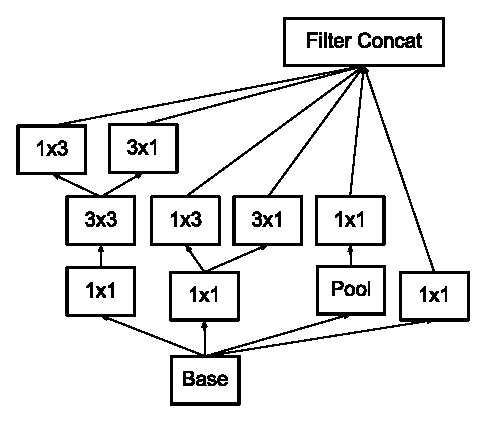
\includegraphics[width=\textwidth]{inception-v3-3}
        \caption{An Inception v3 Block}\label{fig:inception-v3-3}
    \end{subfigure}
    \begin{subfigure}[b]{0.4\textwidth}
        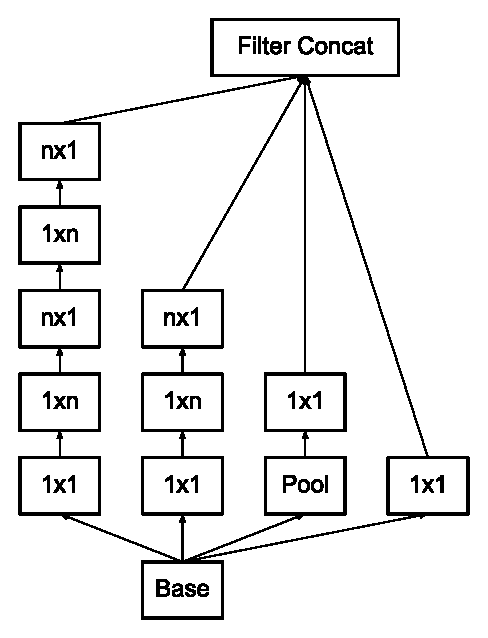
\includegraphics[width=\textwidth]{inception-v3-n}
        \caption{An Inception v3 Block used with \(n=7\)}\label{fig:inception-v3-n}
    \end{subfigure}
\caption{Two variations of Inception v3 blocks }\label{fig:inception-v3}
{Source: \autocite{szegedy2016rethinking}}
\end{figure}



In version two of inception, 5×5 was replaced with 3×3 (as two concatenated 3×3 would have the same receptive field of 5×5)
Also separable convolution is done in this version too early as first layer which produce 64 depth using depth multiplier DM=8.
Beside reduction along the depth, inception v2 introduced reduction along width and height which is called
``Introduced Spatial Factorization'' using
``Asymmetric Convolutions'' that is separating \(k\times k\) kernels into \(k\times 1\) followed by \( 1\times k \).
In Inception v1, all inception blocks were identical while later inception version have many variations of the inception block
one of them having 3×3 followed by 1×1 kernels instead of 3×3 kernel. And another type with 1×1, 7×7, 1×1 then followed by 7×7.
Two variants of this technique is seen in figure \ref{fig:inception-v3}.

Counting layers in inception is tricky and misleading,
because reducing an operator using ``separable operator'' methodology into two or more layers make a less generic filter with more layers.

% TODO: find a better metric to measure depth other than misleading number of layers

\begin{table*}\caption{Comparing all versions of Inception}\label{table:inception-ver-1-4}
\centering
\begin{tabular}{@{}cccccc@{}}
\toprule
Model Name & layers & weights & mults & Top-1 accuracy & Top-5 accuracy \\
\midrule
Inception v1 & 22 & 6.6M & 1,498M & 69.8 & 89.6 \\
Inception v2 & 42 & 11M & 1,934M & 73.9 & 91.8 \\
Inception v3 & 53 & 27M & 5,719M & 78.0 & 93.9 \\
Inception v4 & 81 & 46M & 13,882M & 80.2 & 95.2 \\
Inception ResNet V2 & 130 & 59M & 14,882M & 80.4 & 95.3 \\
\bottomrule
\end{tabular}
\end{table*}

\subsection{Highway Networks}

Deeper networks are more difficult to train due to vanishing gradients, 
a problem which is also faced by Recurrent Neural Networks (RNNs)
that was approached by long short term memory (LSTM) blocks
which uses gates that facilitate information passing from one block to another block as in figure \ref{fig:lstm-chain}.

Inspired by LSTM, Highway Networks\autocite{srivastava2015highway}\autocite{srivastava2015training} 
uses gated information flow in deeper CNNs. Hidden layer output \(H\)
can be suppressed and replaced by passing input \(x\), depending on the value of
a special gate \(T\) which takes a value from zero to one (using sigmoid function)
as in formula \ref{eq:highway}.

\begin{equation}
y = H(x, W_{H} ) \cdot T (x, W_{T} ) + x \cdot (1 - T (x, W_{T} ))
\label{eq:highway}
\end{equation}

By having \(T=0\), the first term will be zero and the second term will be the input \(x\) as is,
that is information bypassing current layer and flow to next deeper layer.


\begin{figure}[!h]
\centering
\includegraphics[width=5in]{lstm-chain}
\caption{An LSTM-block showing gated flow of information in red color}\label{fig:lstm-chain}
{Source: \href{http://colah.github.io/posts/2015-08-Understanding-LSTMs/}{http://colah.github.io}\hfill}
\end{figure}


\subsection{ResNet}

ResNet\autocite{he2016deep}\autocite{he2016identity} is the winner of ILSVRC 2015.
ResNet extends the concept of highway in a more simpler way by just adding input every two layers,
it's like having constant \(T=0.5\) in formula \ref{eq:highway}.

The main idea as in figure {fig:resnet} from first paper\autocite{he2016deep} is to pass the original signal ``as is''
after every two layers with trainable weights using addition and ``ReLU'' (as seen in figure \ref{fig:resnet-block})
then just stack this building unit deeper and deeper.

\begin{figure}[!h]
\centering
    \begin{subfigure}[b]{0.4\textwidth}
        \includegraphics[width=\textwidth]{resnet}
        \caption{ResNet Building Block}\label{fig:resnet-block}
    \end{subfigure}
    \begin{subfigure}[b]{0.4\textwidth}
        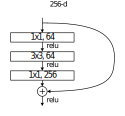
\includegraphics[width=\textwidth]{resnet-bottleneck}
        \caption{ResNet Bottleneck}\label{fig:resnet-bottleneck}
    \end{subfigure}
\caption{ResNet building block}\label{fig:resnet}
{Source: \autocite{he2016deep}\hfill}
\end{figure}

This paper use a form of separable operator reduction called ``bottleneck'' (as in figure \ref{fig:resnet-bottleneck})
which places 1×1 kernel before and after 3×3 kernel.

The second paper\autocite{he2016identity} changes the placement of batch normalization and ReLU as seen in figure \ref{fig:resnet-bn}

And because the original signal is not fading with depth this allowed them to go deeper up to one thousand layers.
Different variation of this design have 50, 101, 152, 200, and even 1000 layers.

ResNet uses 7×7 convolutions with stride of 2, pool 3×3/2 then just repeat the building block of [1×1, 3×3, 1×1 ] many times,
the last 1×1 output volume is 1×1×1000 and it’s followed by average pooling from 2000 to 1000
then fully connected layer to classes.

And like inception, ResNet does not have a layer with most weights,
the weight is well distributed as the heaviest layer in terms of number of parameters
have about 8\% of weights in the 50-layer version (that is the last fully connected layer),
4.7\% in the 101 layer version, 3.9\% in the 151 layers version.

And like inception number of layers is misleading because the use of separable operators.

\begin{figure}[!h]
\centering
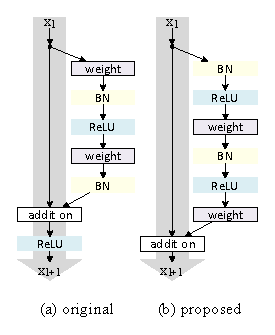
\includegraphics[width=0.48\textwidth]{resnet-bn}
\caption{Placement of Batch normalization in ResNet}\label{fig:resnet-bn}
{Source: \autocite{he2016identity}\hfill}
\end{figure}


\subsection{Inception v4 And Inception-ResNet}

Inception v4 And Inception-ResNet\autocite{szegedy2017inception} are variations of previously discussed Inception
that utilized residual connections in a way similar to ResNet\autocite{he2016deep}

\subsection{DenseNet}
Densely connected convolutional networks (DenseNet)\autocite{huang2016densely},
to counter vanishing gradients as network becomes deeper,
a way for first input is allowed to pass through to deeper layers,
Highway Networks which gates input and optionally pass it to deeper layers
and ResNet which adds input every two layers/blocks,
DenseNet just concatenate signals for all previous layers as in figure \ref{fig:densenet}.

\begin{figure}[!h]
\centering
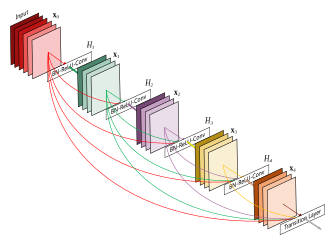
\includegraphics[width=3in]{densenet}
\caption{DenseNet have each layer gets input from all previous layers}\label{fig:densenet}
{Source: \autocite{huang2016densely}\hfill}
\end{figure}


\subsection{MobileNet and SqueezeNet}

MobileNet\autocite{howard2017mobilenets} does not compete on accuracy but on speed.
Similar to SqueezeNet\autocite{iandola2016squeezenet} in the use of the following strategies\autocite{iandola2016squeezenet}\autocite{he2015convolutional}:
Delay down-sampling toward the end of the network,
that is pooling layers and convolutions with strides to get accuracy
which other network put early in the network to reduce number of operations.
Instead they use \(1\times 1\) convolutions instead of more larger \(3\times 3\) 
and reduce the depth of the \(3 \times 3\) filters to reduce number of parameters and operations.

The idea of \(1\times 1\) did not first appear with MobileNet and SqueezeNet,
as it's used heavily in Inception as seen before,
but in MobileNet it's used as replacement of earlier stride to reduce the network computational cost,
MobileNet v1.0 has competitive accuracy compared with inception v1 with half number of parameters.
MobileNet v2.0\autocite{sandler2018inverted} reaches better accuracy than Inception v1 with half the number of parameters.

There are no fully connected layer in SqueezeNet, which is called ``Quantizing FC layer''\autocite{wu2016quantized}.

\subsection{NASNet}

NASNet\autocite{zoph2017learning} has multiple settings, some are small suitable for
mobile applications that competes with MobileNet and Inception v1.
While others has order of magnitude more operations and weights that compete with Inception v4 and ResNet in terms of accuracy. 
Here are two interesting settings on NASNet:

\begin{itemize}
\item NASNet-A (6 @ 4032), 331x331, 88.9M params, 23.8B mults
\item NASNet-A (4 @ 1056), 224x224, 5.3M params, 564M mults
\end{itemize}

The main contribution of NASNet is not their specific network design,
but rather is having that design done by a neural network instead of a human expert.
Another aspect of it, that the training did not happen on ImageNet high resolution images of 1K classes
but rather on a simpler task of classifying tiny images of ten classes (CIFAR-10),
then the architecture is transferred to ImageNet 1k.

\section{Pre-processing}

The bare minimum pre-processing is to resize input image to make it
fit the perceptive field of the network (typically \(224\times 224\) pixels).
Some CNNs have special normalization done to input images,
like subtracting image mean as in VGG\autocite{simonyan2014very},
while others also divide by the standard deviation of the image.
Such transformations should be done in both training phase and prediction phase.

Some pre-processing is done in training phase only to have better generalization, like:
random cropping of a random bounding box in input image, 
random left/right flipping, and random color distorting (brightness, saturation, and contrast).

\section{Stochastic Optimizers}

The factors that affect the efficiency of ANN have been discussed in academia for ages
for example \autocite{lecuniefficient}
(which was part of a book published 1998\autocite{orr1998neural}, that has more recent editions \autocite{orr2012neural}).

There are variations of plain stochastic gradient descent (SDG), the are adaptive and faster to converge like:
SGD momentum\autocite{sutskever2013importance},
Adagrad\autocite{duchi2011adaptive},
Adam\autocite{kingma2014adam},
Adadelta\autocite{zeiler2012adadelta},
and RMSprop\autocite{dozat2016incorporating}\autocite{sutskever2013importance}

PhD. student Sebastian Ruder has made a nice \href{http://sebastianruder.com/optimizing-gradient-descent/}{animation} that compare how they work.

\section{Knowledge Transfer and fine-tuning}

Humans learn multiple tasks at once, and they learn how to generalize,
and how to learn and the learning process is non-stopping continuous streams.
If a computer program that work on a family of tasks each having its own training and
its own experience and its own performance measures, then the computer program is said\autocite{thrun1998learning}
to be capable of ``learning to learn'' if its performance depends on number of tasks (not just a single task).
This field is called multi-task learning and in this type both tasks are trained simultaneously and
one of them enhances the other.

\begin{figure}[!h]
\centering
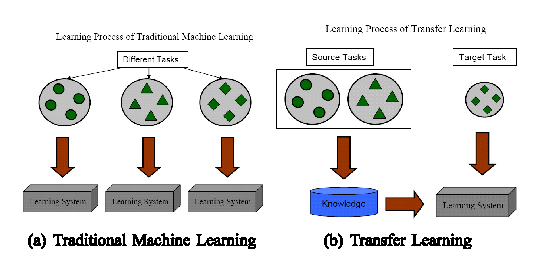
\includegraphics[width=5in]{transfer-learning}
\caption{Transfer-learning}\label{fig:transfer-learning}
{Source: \autocite{pan2010survey}\hfill}
\end{figure}

``Self-taught Learning'' as in \autocite{raina2007self} use unsupervised machine learning to train the machine
how to generalize and construct higher-level features despite the lack of labeled dataset in source task,
and utilize that to in the labeled supervised target task.

Knowledge Transfer is all about reusing some parts from an already solved task and
borrowing knowledge from an already trained and accurate classifier as seen in figure \ref{fig:transfer-learning}.
There are several settings for such process\autocite{pan2010survey} depending on the relation between
source domain \( D_{s} \) and target domain \( D_{t} \), and the relation between
source task \( \tau_{s} \) and target task \( \tau_{t} \) as they can be either the same or similar but different.
Also Knowledge Transfer has to define\autocite{pan2010survey}

\begin{itemize}
\item ``What to transfer?''
\item ``How to transfer?''
\item ``When not to transfer?''
\end{itemize}

The transfer algorithm has to find what parts of knowledge can be transferred across domains and tasks,
then how to actually do the transfer, depending on the availability of labeled training
dataset in either of the domains (source and target).
Domain adaptation\autocite{saenko2010adapting} considered same task on two different but similar domains,
by finding a cross-domain transformation that maps points in source domain to target domain,
as opposed to ``Category Transfer'' which maps labels as in figure \ref{fig:domain-adapt}.

% \autocite{pratt1993discriminability}

\begin{figure}[!h]
\centering
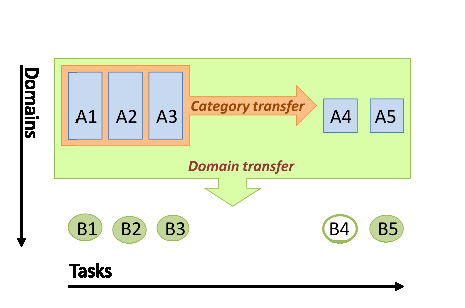
\includegraphics[width=2in]{domain-adapt}
\caption{Difference between ``Category Transfer'' and ``Domain Transfer''.}\label{fig:domain-adapt}
{Source: \autocite{saenko2010adapting}\hfill}
\end{figure}

There are several categorization for the ``how''\autocite{pan2010survey}:

\begin{description}
\item [Instance-transfer] To re-weight some labeled data in the source domain for use in the target domain.
\item [Feature-representation-transfer] To find a ``good'' feature representation that reduces difference between the source and the target
domains and the error of classification and regression models.
\item [Parameter-transfer] Discover shared parameters or priors between the source domain and target domain models, which can benefit for transfer learning
\item [Relational-knowledge-transfer] Build mapping of relational knowledge between the source domain and the target domains. Both domains are relational domains and i.i.d assumption is relaxed in each domain.
\item [Architecture transfer] train an \gls{rnn} to find best architecture on a simple task, transfer architecture to difficult task as in NASNet\autocite{zoph2017learning}
\end{description}

% TODO: do we need to talk about meta learner / fast-learner. 

Other types of transfer learning have a prior (not simultaneous) knowledge (that is possibly static)
in one task that is used to induce knowledge in another task both in same domain and feature space
which is the type that this research would focus on where source domain and target domain are the same
(which is the input image and its pixels are the feature).
Source task is the ImageNet classification task from \gls{ilsvrc},
and the prior knowledge is one of the pre-trained state-of-the-art models.
Target task is to classify different dataset obtained from the e-Commerce platform or the fine-grained datasets of flowers,
dogs, birds, food.

Fine-tuning\autocite{zeng2016gated}\autocite{ouyang2016factors}\autocite{sharif2014cnn} is a type of ``Parameter-transfer''.
Taking an ``off-the-shelf''\autocite{sharif2014cnn} pre-trained state of the art \gls{cnn} model
then re-fit it on different task by taking all weights except those in last fully connected layer 
or by adding an \gls{svm} after last convolution (called CNN-SVM).
This works because several researches\autocite{donahue2014decaf}\autocite{girshick2014rich}\autocite{oquab2014learning}
have shown and even visualized\autocite{zeiler2014visualizing} that when moving toward the end of the neural network,
the deeper the more high-level features, moving from low primitives to complete objects or entities (eyes, faces, ..etc.)

% off-topic \autocite{taigman2014deepface}, \autocite{toshev2014deeppose}, \autocite{zhang2014panda}

Some other methods utilize knowledge from unlabeled datasets or noisy datasets
and transfer knowledge to enhancing labeled but small dataset as in papers\autocite{reed2014training}\autocite{sukhbaatar2014training}\autocite{sukhbaatar2014learning}\autocite{van2015building}

A different approach was done by Google Brain Team in their paper \autocite{bello2017neural}
as they proposed a way for ``Architecture Search''
but that was expensive for large database, that's why in their other paper\autocite{zoph2017learning}
used transferred knowledge from a very simple problem that is CIFAR-10 dataset to
the state-of-the-art difficult problem ImageNet\autocite{deng2009imagenet} dataset.
They did not transfer weights, as they train from scratch after transfer,
they transfer architecture and design not knowledge which resulted in NASNet discussed before.

